% Created by tikzDevice version 0.12.6 on 2025-05-24 13:24:01
% !TEX encoding = UTF-8 Unicode
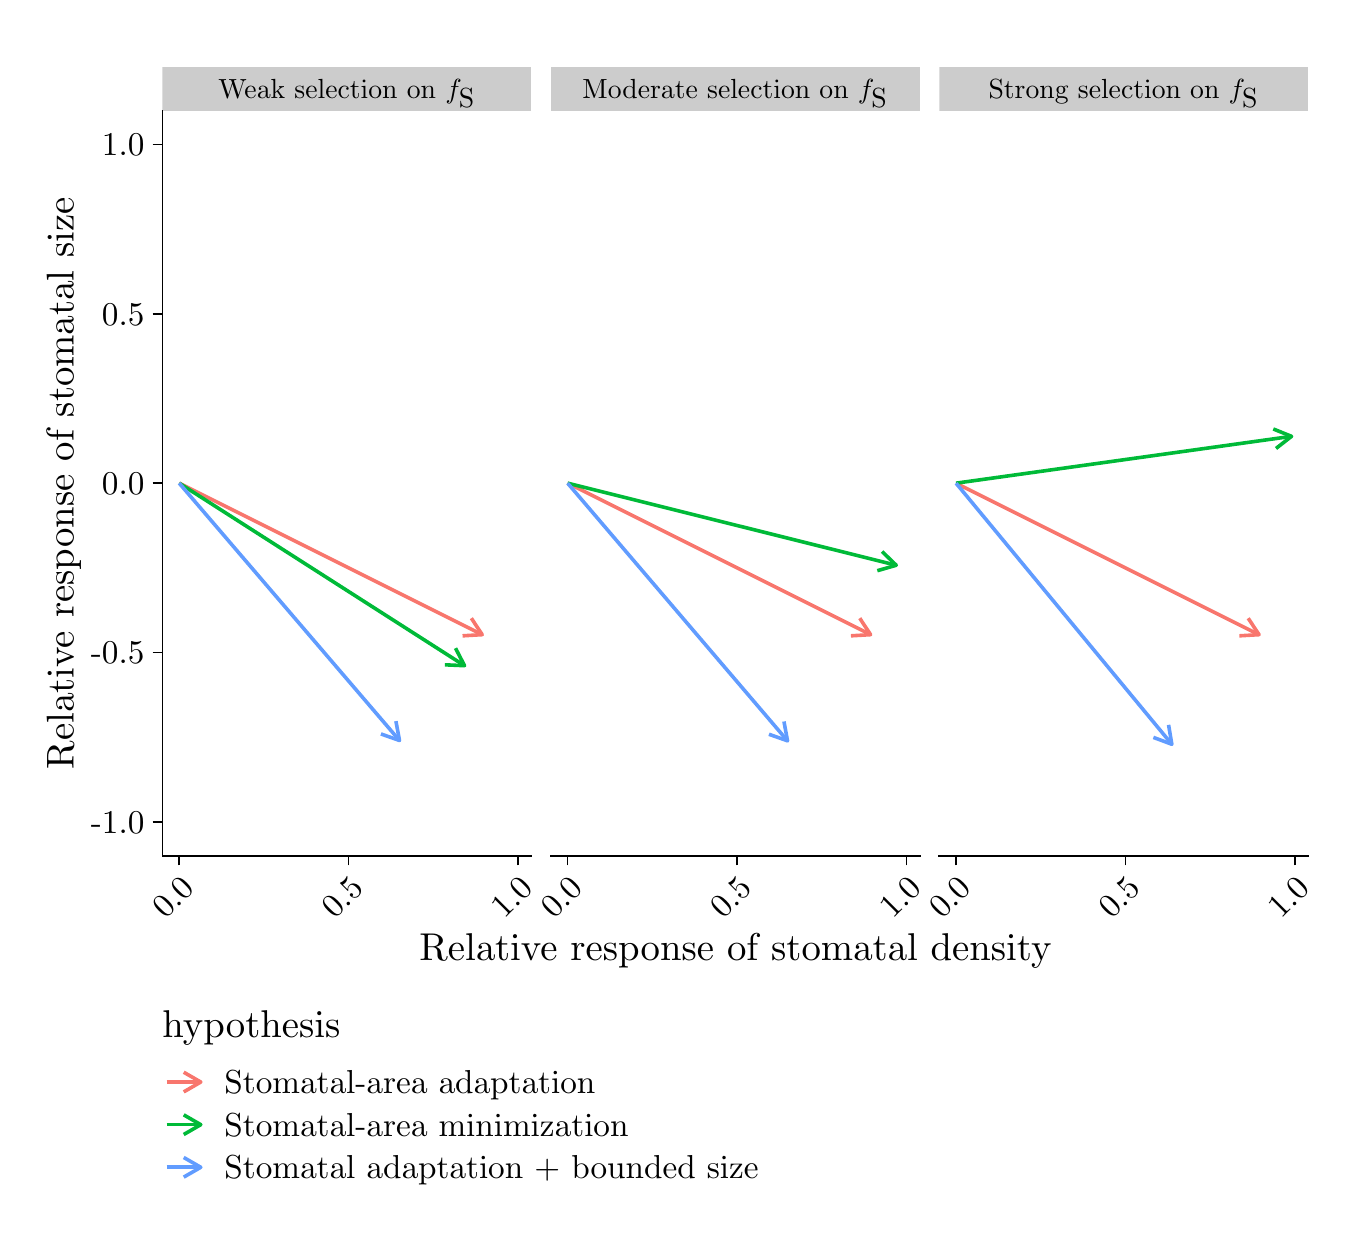
\begin{tikzpicture}[x=1pt,y=1pt]
\definecolor{fillColor}{RGB}{255,255,255}
\path[use as bounding box,fill=fillColor,fill opacity=0.00] (0,0) rectangle (469.75,433.62);
\begin{scope}
\path[clip] ( 48.69,134.38) rectangle (182.05,403.67);
\definecolor{drawColor}{RGB}{248,118,109}

\path[draw=drawColor,line width= 1.3pt,line join=round] ( 54.75,269.02) -- (164.24,214.28);

\path[draw=drawColor,line width= 1.3pt,line join=round] (157.14,213.86) --
	(164.24,214.28) --
	(160.32,220.22);
\definecolor{drawColor}{RGB}{0,186,56}

\path[draw=drawColor,line width= 1.3pt,line join=round] ( 54.75,269.02) -- (157.87,203.07);

\path[draw=drawColor,line width= 1.3pt,line join=round] (150.77,203.39) --
	(157.87,203.07) --
	(154.60,209.39);
\definecolor{drawColor}{RGB}{97,156,255}

\path[draw=drawColor,line width= 1.3pt,line join=round] ( 54.75,269.02) -- (134.36,176.04);

\path[draw=drawColor,line width= 1.3pt,line join=round] (127.65,178.41) --
	(134.36,176.04) --
	(133.06,183.03);
\end{scope}
\begin{scope}
\path[clip] (189.05,134.38) rectangle (322.40,403.67);
\definecolor{drawColor}{RGB}{248,118,109}

\path[draw=drawColor,line width= 1.3pt,line join=round] (195.11,269.02) -- (304.59,214.28);

\path[draw=drawColor,line width= 1.3pt,line join=round] (297.49,213.86) --
	(304.59,214.28) --
	(300.67,220.22);
\definecolor{drawColor}{RGB}{0,186,56}

\path[draw=drawColor,line width= 1.3pt,line join=round] (195.11,269.02) -- (313.86,239.36);

\path[draw=drawColor,line width= 1.3pt,line join=round] (307.02,237.40) --
	(313.86,239.36) --
	(308.75,244.30);
\definecolor{drawColor}{RGB}{97,156,255}

\path[draw=drawColor,line width= 1.3pt,line join=round] (195.11,269.02) -- (274.57,175.92);

\path[draw=drawColor,line width= 1.3pt,line join=round] (267.87,178.29) --
	(274.57,175.92) --
	(273.28,182.91);
\end{scope}
\begin{scope}
\path[clip] (329.40,134.38) rectangle (462.76,403.67);
\definecolor{drawColor}{RGB}{248,118,109}

\path[draw=drawColor,line width= 1.3pt,line join=round] (335.46,269.02) -- (444.95,214.28);

\path[draw=drawColor,line width= 1.3pt,line join=round] (437.84,213.86) --
	(444.95,214.28) --
	(441.03,220.22);
\definecolor{drawColor}{RGB}{0,186,56}

\path[draw=drawColor,line width= 1.3pt,line join=round] (335.46,269.02) -- (456.69,285.94);

\path[draw=drawColor,line width= 1.3pt,line join=round] (451.08,281.57) --
	(456.69,285.94) --
	(450.10,288.61);
\definecolor{drawColor}{RGB}{97,156,255}

\path[draw=drawColor,line width= 1.3pt,line join=round] (335.46,269.02) -- (413.44,174.67);

\path[draw=drawColor,line width= 1.3pt,line join=round] (406.78,177.16) --
	(413.44,174.67) --
	(412.26,181.69);
\end{scope}
\begin{scope}
\path[clip] ( 48.69,403.67) rectangle (182.05,419.50);
\definecolor{fillColor}{gray}{0.80}

\path[fill=fillColor] ( 48.69,403.67) rectangle (182.05,419.50);
\definecolor{drawColor}{RGB}{0,0,0}

\node[text=drawColor,anchor=base,inner sep=0pt, outer sep=0pt, scale=  1.00] at (115.37,408.14) {Weak selection on $f_\textrm{S}$};
\end{scope}
\begin{scope}
\path[clip] (189.05,403.67) rectangle (322.40,419.50);
\definecolor{fillColor}{gray}{0.80}

\path[fill=fillColor] (189.05,403.67) rectangle (322.40,419.50);
\definecolor{drawColor}{RGB}{0,0,0}

\node[text=drawColor,anchor=base,inner sep=0pt, outer sep=0pt, scale=  1.00] at (255.72,408.14) {Moderate selection on $f_\textrm{S}$};
\end{scope}
\begin{scope}
\path[clip] (329.40,403.67) rectangle (462.76,419.50);
\definecolor{fillColor}{gray}{0.80}

\path[fill=fillColor] (329.40,403.67) rectangle (462.75,419.50);
\definecolor{drawColor}{RGB}{0,0,0}

\node[text=drawColor,anchor=base,inner sep=0pt, outer sep=0pt, scale=  1.00] at (396.08,408.14) {Strong selection on $f_\textrm{S}$};
\end{scope}
\begin{scope}
\path[clip] (  0.00,  0.00) rectangle (469.75,433.62);
\definecolor{drawColor}{RGB}{0,0,0}

\path[draw=drawColor,line width= 0.6pt,line join=round,line cap=rect] ( 48.69,134.38) --
	(182.05,134.38);
\end{scope}
\begin{scope}
\path[clip] (  0.00,  0.00) rectangle (469.75,433.62);
\definecolor{drawColor}{RGB}{0,0,0}

\path[draw=drawColor,line width= 0.6pt,line join=round] ( 54.75,130.88) --
	( 54.75,134.38);

\path[draw=drawColor,line width= 0.6pt,line join=round] (115.96,130.88) --
	(115.96,134.38);

\path[draw=drawColor,line width= 0.6pt,line join=round] (177.16,130.88) --
	(177.16,134.38);
\end{scope}
\begin{scope}
\path[clip] (  0.00,  0.00) rectangle (469.75,433.62);
\definecolor{drawColor}{RGB}{0,0,0}

\node[text=drawColor,rotate= 45.00,anchor=base east,inner sep=0pt, outer sep=0pt, scale=  1.20] at ( 60.60,122.03) {0.0};

\node[text=drawColor,rotate= 45.00,anchor=base east,inner sep=0pt, outer sep=0pt, scale=  1.20] at (121.80,122.03) {0.5};

\node[text=drawColor,rotate= 45.00,anchor=base east,inner sep=0pt, outer sep=0pt, scale=  1.20] at (183.00,122.03) {1.0};
\end{scope}
\begin{scope}
\path[clip] (  0.00,  0.00) rectangle (469.75,433.62);
\definecolor{drawColor}{RGB}{0,0,0}

\path[draw=drawColor,line width= 0.6pt,line join=round,line cap=rect] (189.05,134.38) --
	(322.40,134.38);
\end{scope}
\begin{scope}
\path[clip] (  0.00,  0.00) rectangle (469.75,433.62);
\definecolor{drawColor}{RGB}{0,0,0}

\path[draw=drawColor,line width= 0.6pt,line join=round] (195.11,130.88) --
	(195.11,134.38);

\path[draw=drawColor,line width= 0.6pt,line join=round] (256.31,130.88) --
	(256.31,134.38);

\path[draw=drawColor,line width= 0.6pt,line join=round] (317.51,130.88) --
	(317.51,134.38);
\end{scope}
\begin{scope}
\path[clip] (  0.00,  0.00) rectangle (469.75,433.62);
\definecolor{drawColor}{RGB}{0,0,0}

\node[text=drawColor,rotate= 45.00,anchor=base east,inner sep=0pt, outer sep=0pt, scale=  1.20] at (200.95,122.03) {0.0};

\node[text=drawColor,rotate= 45.00,anchor=base east,inner sep=0pt, outer sep=0pt, scale=  1.20] at (262.15,122.03) {0.5};

\node[text=drawColor,rotate= 45.00,anchor=base east,inner sep=0pt, outer sep=0pt, scale=  1.20] at (323.36,122.03) {1.0};
\end{scope}
\begin{scope}
\path[clip] (  0.00,  0.00) rectangle (469.75,433.62);
\definecolor{drawColor}{RGB}{0,0,0}

\path[draw=drawColor,line width= 0.6pt,line join=round,line cap=rect] (329.40,134.38) --
	(462.76,134.38);
\end{scope}
\begin{scope}
\path[clip] (  0.00,  0.00) rectangle (469.75,433.62);
\definecolor{drawColor}{RGB}{0,0,0}

\path[draw=drawColor,line width= 0.6pt,line join=round] (335.46,130.88) --
	(335.46,134.38);

\path[draw=drawColor,line width= 0.6pt,line join=round] (396.67,130.88) --
	(396.67,134.38);

\path[draw=drawColor,line width= 0.6pt,line join=round] (457.87,130.88) --
	(457.87,134.38);
\end{scope}
\begin{scope}
\path[clip] (  0.00,  0.00) rectangle (469.75,433.62);
\definecolor{drawColor}{RGB}{0,0,0}

\node[text=drawColor,rotate= 45.00,anchor=base east,inner sep=0pt, outer sep=0pt, scale=  1.20] at (341.31,122.03) {0.0};

\node[text=drawColor,rotate= 45.00,anchor=base east,inner sep=0pt, outer sep=0pt, scale=  1.20] at (402.51,122.03) {0.5};

\node[text=drawColor,rotate= 45.00,anchor=base east,inner sep=0pt, outer sep=0pt, scale=  1.20] at (463.71,122.03) {1.0};
\end{scope}
\begin{scope}
\path[clip] (  0.00,  0.00) rectangle (469.75,433.62);
\definecolor{drawColor}{RGB}{0,0,0}

\path[draw=drawColor,line width= 0.6pt,line join=round,line cap=rect] ( 48.69,134.38) --
	( 48.69,403.67);
\end{scope}
\begin{scope}
\path[clip] (  0.00,  0.00) rectangle (469.75,433.62);
\definecolor{drawColor}{RGB}{0,0,0}

\node[text=drawColor,anchor=base east,inner sep=0pt, outer sep=0pt, scale=  1.20] at ( 42.19,142.49) {-1.0};

\node[text=drawColor,anchor=base east,inner sep=0pt, outer sep=0pt, scale=  1.20] at ( 42.19,203.69) {-0.5};

\node[text=drawColor,anchor=base east,inner sep=0pt, outer sep=0pt, scale=  1.20] at ( 42.19,264.89) {0.0};

\node[text=drawColor,anchor=base east,inner sep=0pt, outer sep=0pt, scale=  1.20] at ( 42.19,326.10) {0.5};

\node[text=drawColor,anchor=base east,inner sep=0pt, outer sep=0pt, scale=  1.20] at ( 42.19,387.30) {1.0};
\end{scope}
\begin{scope}
\path[clip] (  0.00,  0.00) rectangle (469.75,433.62);
\definecolor{drawColor}{RGB}{0,0,0}

\path[draw=drawColor,line width= 0.6pt,line join=round] ( 45.19,146.62) --
	( 48.69,146.62);

\path[draw=drawColor,line width= 0.6pt,line join=round] ( 45.19,207.82) --
	( 48.69,207.82);

\path[draw=drawColor,line width= 0.6pt,line join=round] ( 45.19,269.02) --
	( 48.69,269.02);

\path[draw=drawColor,line width= 0.6pt,line join=round] ( 45.19,330.23) --
	( 48.69,330.23);

\path[draw=drawColor,line width= 0.6pt,line join=round] ( 45.19,391.43) --
	( 48.69,391.43);
\end{scope}
\begin{scope}
\path[clip] (  0.00,  0.00) rectangle (469.75,433.62);
\definecolor{drawColor}{RGB}{0,0,0}

\node[text=drawColor,anchor=base,inner sep=0pt, outer sep=0pt, scale=  1.40] at (255.72, 96.40) {Relative response of stomatal density};
\end{scope}
\begin{scope}
\path[clip] (  0.00,  0.00) rectangle (469.75,433.62);
\definecolor{drawColor}{RGB}{0,0,0}

\node[text=drawColor,rotate= 90.00,anchor=base,inner sep=0pt, outer sep=0pt, scale=  1.40] at ( 16.64,269.02) {Relative response of stomatal size};
\end{scope}
\begin{scope}
\path[clip] (  0.00,  0.00) rectangle (469.75,433.62);
\definecolor{drawColor}{RGB}{0,0,0}

\node[text=drawColor,anchor=base west,inner sep=0pt, outer sep=0pt, scale=  1.40] at ( 48.69, 68.68) {hypothesis};
\end{scope}
\begin{scope}
\path[clip] (  0.00,  0.00) rectangle (469.75,433.62);
\definecolor{drawColor}{RGB}{248,118,109}

\path[draw=drawColor,line width= 1.3pt,line join=round] ( 50.23, 52.62) -- ( 62.55, 52.62);

\path[draw=drawColor,line width= 1.3pt,line join=round] ( 56.39, 49.06) --
	( 62.55, 52.62) --
	( 56.39, 56.17);
\end{scope}
\begin{scope}
\path[clip] (  0.00,  0.00) rectangle (469.75,433.62);
\definecolor{drawColor}{RGB}{0,186,56}

\path[draw=drawColor,line width= 1.3pt,line join=round] ( 50.23, 37.22) -- ( 62.55, 37.22);

\path[draw=drawColor,line width= 1.3pt,line join=round] ( 56.39, 33.66) --
	( 62.55, 37.22) --
	( 56.39, 40.77);
\end{scope}
\begin{scope}
\path[clip] (  0.00,  0.00) rectangle (469.75,433.62);
\definecolor{drawColor}{RGB}{97,156,255}

\path[draw=drawColor,line width= 1.3pt,line join=round] ( 50.23, 21.82) -- ( 62.55, 21.82);

\path[draw=drawColor,line width= 1.3pt,line join=round] ( 56.39, 18.26) --
	( 62.55, 21.82) --
	( 56.39, 25.37);
\end{scope}
\begin{scope}
\path[clip] (  0.00,  0.00) rectangle (469.75,433.62);
\definecolor{drawColor}{RGB}{0,0,0}

\node[text=drawColor,anchor=base west,inner sep=0pt, outer sep=0pt, scale=  1.20] at ( 71.09, 48.49) {Stomatal-area adaptation};
\end{scope}
\begin{scope}
\path[clip] (  0.00,  0.00) rectangle (469.75,433.62);
\definecolor{drawColor}{RGB}{0,0,0}

\node[text=drawColor,anchor=base west,inner sep=0pt, outer sep=0pt, scale=  1.20] at ( 71.09, 33.09) {Stomatal-area minimization};
\end{scope}
\begin{scope}
\path[clip] (  0.00,  0.00) rectangle (469.75,433.62);
\definecolor{drawColor}{RGB}{0,0,0}

\node[text=drawColor,anchor=base west,inner sep=0pt, outer sep=0pt, scale=  1.20] at ( 71.09, 17.69) {Stomatal adaptation + bounded size};
\end{scope}
\end{tikzpicture}
